\subsection{Data Formats} \label{sec:dataformat}

The data format is a part of the process of serialization, which enables data storage in a file, transmission over the Internet, and reconstruction in a different environment. Serialization is the process of converting the state of an object into a stream of bytes, which later can be deserialized by rebuilding the stream of bytes to the original object. There are several data serialization formats; however, JavaScript Object Notation (JSON) and eXtensible Markup Language (XML) are the two most common data serialization formats. This section discuss these formats. In the end, we compare them and choose the format that meets the criteria of being compact, human-readable, and universal. 

\subsubsection{JSON}
JSON or JavaScript Object Notation is a light-weight and human-readable format that is commonly used for interchanging data on the web. The format is a text-based solution where the data structure is built on two structures: a collection of name-value pairs (known as objects) and ordered list of values (known as arrays). The JSON format is language-independent and the data structure universally recognized \cite{jsonorg, jsonvxml}. However, it is limited to a few predefined data types (i.e., string, number, boolean, object, array, and null), and extending the data type has to be done with the preliminary types. 

\begin{lstlisting}[language=json, caption={}, captionpos=b]
{
    "user": {
        "firstname": "Ola"
        "lastname": "Nordmann"
    }
}
\end{lstlisting}

\subsubsection{XML}
XML or eXtensible Markup Language is a simple and flexible format derived from Standard Generalized Markup Language (SGML), developed by the XML Working Group under the World Wide Web Consortium (W3C). An XML document consists of markups called tags, which are containers that describe and organize the enclosed data. The tag starts with \verb|<| and ends with \verb|>|; the content is placed between an opening tag and a closing tag. \cite{w3xml, jsonvxml} XML provides mechanisms to define custom data types, using existing data types as a starting point, making it extensible for future data. 

\begin{lstlisting}[language=json, caption={}, captionpos=b]
<user>
    <firstname>Ola</firstname>
    <lastname>Nordmann</lastname>
</user>
\end{lstlisting}

\subsubsection{Comparing}
With the study conducted by Saurabh and D’Souza \cite{jsonvxml}, we compare JSON and XML features and performance. There are apparent differences in the two data formats which affect the overall readability, extensibility, bandwidth performance, and ease of mapping. XML documents are easy to read, while JSON is obscure due to the parenthesis delimiters. XML allows for extended data types, while JSON is limited to a few data types. XML takes more bandwidth due to the metadata overhead, while JSON data is compact and use less amount of bandwidth.

Moreover, a few benchmarks were conducted to measure memory footprint and parsing runtime when serializing and deserializing JSON and XML data. From the conclusion,  in terms of memory footprint and parsing runtime, JSON performances better than XML, but at the cost of readability and flexibility. While these format structures are applicable for transmitting data, choosing a format that is compact, human-readable, and a standard format that is extensible and scalable for future data is essential. In our design, we use the JSON format for transmission of the data.

\begin{figure}
    \centering
    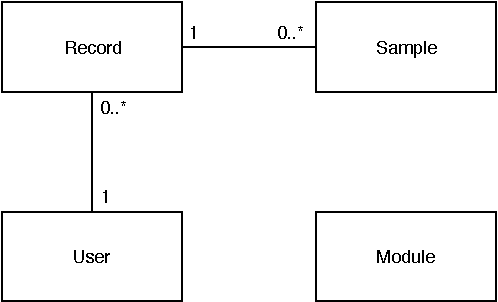
\includegraphics[scale=0.8]{images/DataEntries.pdf}
    \caption{The data model and relationship for the entities in the application: a record has zero to many samples, while a sample only can have one record. A record can have one user, while a user can have many records. A module has no relationship with the other entities.}
    \label{fig:dataentries}
\end{figure}

\subsection{Data Entities}\label{des:dataentity}
Data entities are objects (e.g., things, persons, or places) that the system models and stores information about. In Section \ref{soc:storage}, we introduced four data entities in the application (i.e., record, sample, module, and user). In Figure \ref{fig:dataentries}, the relations between the data entities are shown. The record entity and sample entity store information about the recording session\footnote{the ongoing process of collecting data from the sensor sources and storing the samples (data packets) in the database.} and are separated into two individual entities in order to reduce data redundancy and improve data integrity. The sample entity has a reference to its record entity so they can be associated with each other. The user entity store biometrical information related to the user (i.e., patients). Also, a record entity contains the state of the user's biometrical information at the time of the recording. In other words, the user's biometrical information can change over time (e.g.,  weight changes); therefore, capturing the exact biometrical information at the time of the recording is essential in the context of detecting sleeping illnesses with relation to the biometrical information.  A module entity is independent of the other data entities and stores information about the name and the package name of the module-application. The package name is used to locate and launch the module-application. 

In the following sections, we present the properties of each data entity in Nidra; storage structure of the entities, and illustration of the data structure for each entity.  



\subsubsection{Record Entity} \label{ssec:record}

The table for the record entity in the database stores metadata (e.g., elapsed time of recording, number of samples, user's biometrical data) related to a recording session. In Table 4.1, we present the information (fields) the record entity contains, which can be described as: 
\begin{itemize}
    \item \verb|ID|: Unique identification of a record, also a primary key for the entry.
    \item \verb|Name|: A name of the record to easily recognize the recording.
    \item \verb|Description|: A summary of the recording session provided by the user. It can be used to briefly describe how the recording session felt (e.g., any abnormalities during the sleep).
    \item \verb|MonitorTime|: The recording session duration in milliseconds.
    \item \verb|Rating|: Giving a rating on how the sleeping session felt, in a range between 0-5. 
    \item \verb|User|: User's biometrical information encoded into a JSON string format, in order to capture the state of the user at recording. 
    \item \verb|CreatedAt|: Date of creation of the recording in milliseconds (since January 1, 1970, 00:00:00 GMT).
    \item \verb|UpdatedAt|: Date of update of the recording in milliseconds (since January 1, 1970, 00:00:00 GMT).
\end{itemize}

\begin{table}[!h]
\begin{center}
\scalebox{0.75}{
\begin{tabular}{ |c|c|c|c|c|c|c|c| } 
\hline
\textbf{id} & \textbf{name} & \textbf{description} & \textbf{monitorTime} & \textbf{rating} & \textbf{user} & \textbf{createdAt} & \textbf{updatedAt} \\
\hline
1 & Record \#1 & - & 5963088 & 2.5 & \{...\} & 1554406256000 & 1554406256000  \\ 
\hline
\end{tabular}}
\caption{Example entry in the record table.}
\end{center}
\end{table}





\subsubsection{Sample Entity} \label{ssec:sample}
The table for the sample entity contains a single sensor reading (data packet) sent from the sensor source. Sample entity are stored separated from a record entity; however, they are linked (foreign key) with their corresponding record entity. In Table 4.2, we present the information (fields) the sample entity contains, which can be described as: 

\begin{itemize}
    \item \verb|ID|: Unique identification of a sample, also a primary key for the entry.
    \item \verb|RecordID|: An identification to its corresponding record, also a foreign key. 
    \item \verb|ExplicitTS|: Timestamp of sample arrival based on the time in the sensor. 
    \item \verb|ImplicitTS|: Timestamp of sample arrival based on the time on the device. 
    \item \verb|Sample|: Sensor reading contains metadata and data according to Flow sensor.
\end{itemize}

\begin{table}[!h]
\begin{center}
\scalebox{0.60}{
\begin{tabular}{ |c|c|c|c|c| } 
\hline
\textbf{id} & \textbf{recordId} & \textbf{explicitTS} & \textbf{implicitTS} & \textbf{sample} \\
\hline
1 & 1 & 1554393086000 & 1554400286000 & Time=0ms, deltaT=100, data=1906,1891,1884,1881,1876,1718,1690 \\ 
\hline
\end{tabular}}
\caption{Example entry in the sample table.}
\end{center}
\end{table}



\subsubsection{Module Entity} \label{ssec:module}
The table for the module entity contains metadata of the module added by the user in the application. In Table 4.3, we present the information (fields) the module entity contains, which can be described as:
\begin{itemize}
    \item \verb|ID|: Unique identification of a module, also a primary key for the entry.
    \item \verb|Name|: The name of the module-application.
    \item \verb|PackageName|: The package name of the module-application, such that it can be launched from Nidra. 
\end{itemize}

\begin{table}[!h]
\begin{center}
\scalebox{0.8}{
\begin{tabular}{ |c|c|c| } 
\hline
\textbf{id} & \textbf{name} & \textbf{packageName} \\
\hline
1 & OSA Predicter & com.package.osa\_predicter \\ 
\hline
\end{tabular}}
\caption{Example entry in the module table.}
\end{center}
\end{table}


\subsubsection{User Entity} \label{ssec:user}
The user of the application is the patient, which provides biometrical data (e.g., weight, height, and age). The biometrical data is part of the application to enrich the record. The record captures the biometrical state of the user at the time of the recording. In Nidra, the user entity is not a part of the database, but stored as an object on the mobile device. The design decision of this choice is because the application is limited to one user at the time, and it makes it convenient to capture the state of the object of the given time of recording. It is possible to create a table in the database for the user entity, and for each time the user changes the biometrical data insert it is a separate entry in the database. The record could then have a reference to the latest user entry. However, that increases the complexity of the system, and as of now, the design of the application is to store the user's biometrical data into an object on the device. 

In the listing below, we present the structure of the user entity. In Nidra, the user entity is stored as an object and structured as a JSON format containing biometrical data related to the user: 
\begin{itemize}
    \item \verb|Name|: A string that contains the name of of the patient.
    \item \verb|Age|: An integer with the age of the patient.
    \item \verb|Gender|: A string that contains the gender of the patient.
    \item \verb|Weight|: An integer with the weight of the patient in kilograms.
    \item \verb|Height|: An integer with the height of the patient in centimeters.
\end{itemize}

\begin{figure}[!h]
\begin{lstlisting}[language=json, caption={}, captionpos=b]
{
    "user": {
        "name": "Ola Nordmann",
        "age": 50,
        "gender": "Male",
        "height": 180,
        "weight: 60
    }
}
\end{lstlisting}
\end{figure}



\subsection{Data Packets}\label{design:datapackets}
Data packets are parcels of data that Nidra receives from external applications (e.g., data streams dispatching module) or send to other application (e.g., by sharing the records on the device). This section presents the format of the records and corresponding samples that are sent across applications (e.g., the data is encoded into a file, and the user can select preferred media, such as e-mail), and presents the data packets forwarded by the data streams dispatching module upon data acquisition from the Flow sensor.

\subsubsection{Sharing}

In \Cref{sec:design_sharing}, a proposal for the structure of exporting and importing data is discussed. Two of the components (\verb|Parse Formatted Content| and \verb|Format File|) use JSON to either encode or decode the data. Listing 4.1 illustrates the content of the encoded data from the application to gain a broader understanding of how the data format looks. To summarize, the JSON string contains an object of record that encompasses the metadata of the recording session, as well as the state of biometrical data of the user. Besides the record object, there is an array of sample objects, where each sample object contains a single sensor reading from the Flow sensor. 

\begin{lstlisting}[language=json, caption={A JSON string object that contains the record which has metadata from the recording session (including the biometrical data of the user), and a list of samples (where each samples contains a single sensor reading).}, captionpos=b]
{
    "record":{  
        "id": 1,
        "name": "Record 1",
        "rating": 2.5,
        "description": "",
        "nrSamples": 6107,
        "monitorTime": 5963088,
        "createdAt": "Apr 4, 2019 9:30:56 PM",
        "updatedAt": "Apr 4, 2019 9:30:56 PM",
        "user": {  
            "age": 50,
            "createdAt": "---",
            "gender": "Male",
            "height": 180,
            "name": "Ola Nordmann",
            "weight": 60
        }
    },
    "samples": [  
        {  
            "explicitTS":"Apr 4, 2019 5:51:26 PM",
            "implicitTS":"Apr 4, 2019 7:51:26 PM",
            "recordId":1,
            "sample":"Time=0ms, deltaT=100, data=1906,1891,1884,1881,1876,1718,1690"
        },
        ...
    ]
}
\end{lstlisting}

\subsubsection{Single Sensor Reading}

Listing 4.2 presents a single sensor reading from the Flow sensor sent from the data streams dispatching module. The \verb|id| is assigned by the data streams dispatching module to identify the subscriber application with the corresponding sensor source. Moreover, the \verb|time| is assigned by the internal timer of the Flow sensor. Also, the \verb|value| is the data sent from the Flow sensor, which encompasses time, delta, and data. However, we are most interested in extracting the data values from the reading. 

\begin{lstlisting}[language=json, caption={Encompasses a single sample received from the Flow sensor.}, captionpos=b]
{
    "id":"1-0",
    "value":"Time=2100ms, deltaT=100, data=1869,1873,1883,1864,1871,1870,1870",
    "time":"2019-07-29T18:20:58.997+0000"
}
\end{lstlisting}


